\documentclass[tikz, border=5]{standalone}

\begin{document}
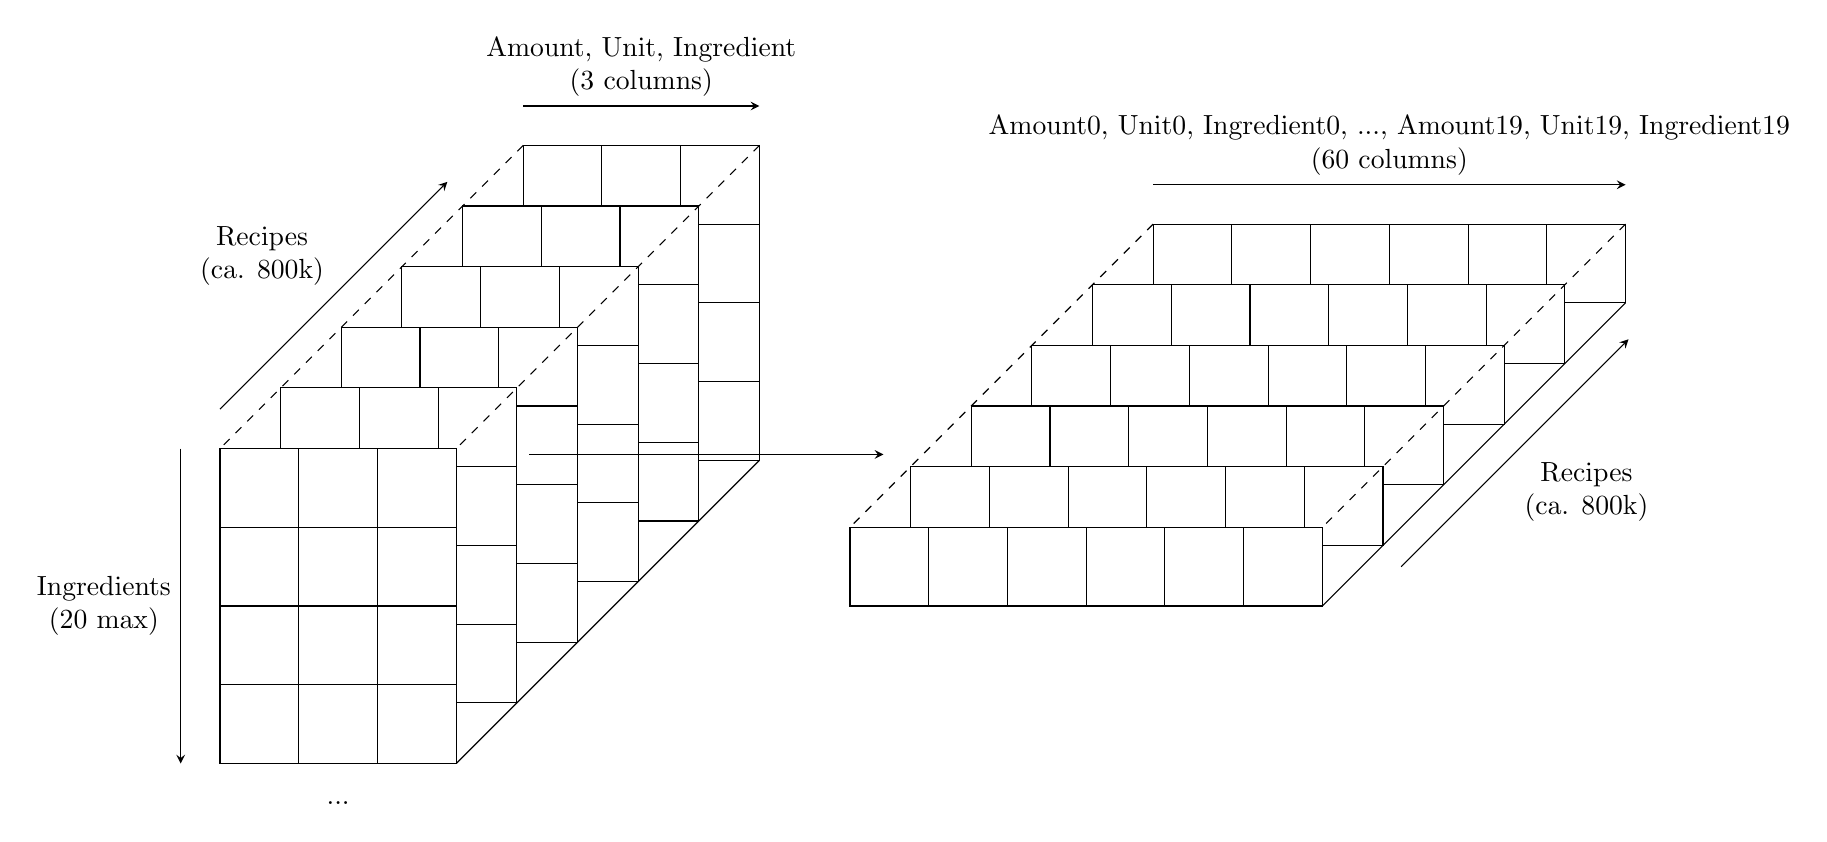
\begin{tikzpicture}[>=stealth]


\draw (0, 0, 0) -- (0, 0, 10) (3, 0, 0) -- (3, 0, 10);
\foreach \z in {0, 2, 4, 6, 8, 10} 
	\foreach \x in {0,...,2}
  		\foreach \y in {0,...,3}
    		\filldraw [fill=white] (\x, \y, \z) -- (\x+1, \y, \z) -- (\x+1, \y+1, \z) --
      			(\x, \y+1, \z) -- cycle (\x+.5, \y+.5, \z) node [yslant=tan(15)] {};
\draw [dashed] (0, 4, 0) -- (0, 4, 10) (3, 4, 0) -- (3, 4, 10);
\draw [->] (0, 4.5, 0)  -- (3, 4.5, 0)   node [midway, above, align=center] {Amount, Unit, Ingredient\\(3 columns)};
\draw [->] (-.5, 4, 10)  -- (-.5, 0, 10)   node [midway, left, align=center] {Ingredients\\(20 max)};
\draw [->] (0, 4.5, 10) -- (0, 4.5, 2.5) node [midway, above left, align=center] {Recipes\\(ca. 800k)};
\draw (1.5,-0.5,10) node {...}; 


\draw [->] (2, 2, 5) -- (6.5, 2, 5);

\draw (8, 2, 0) -- (8, 2, 10) (14, 2, 0) -- (14, 2, 10);
\foreach \z in {0, 2, 4, 6, 8, 10} 
	\foreach \x in {8,...,13}
  		\foreach \y in {2,...,2}
    		\filldraw [fill=white] (\x, \y, \z) -- (\x+1, \y, \z) -- (\x+1, \y+1, \z) --
      			(\x, \y+1, \z) -- cycle (\x+.5, \y+.5, \z) node [yslant=tan(15)] {};
\draw [dashed] (8, 3, 0) -- (8, 3, 10) (14, 3, 0) -- (14, 3, 10);
\draw [->] (8, 3.5, 0)  -- (14, 3.5, 0)   node [midway, above, align=center] {Amount0, Unit0, Ingredient0, ..., Amount19, Unit19, Ingredient19 \\ (60 columns)};
\draw [->] (15, 2.5, 10) -- (15, 2.5, 2.5) node [midway, below right, align=center] {Recipes\\(ca. 800k)};

\end{tikzpicture}%	
\end{document}